\chapter{Concept}
\label{chap:concept}

The following chapter discusses all conceptual work that went into creating Tinzenite.
We will first give an overview of the basic goals of the work created by this thesis.
Next we will expand on the goals by discussing the features we would like Tinzenite to have and defining their scope.
These will be based in part on the existing solutions discussed in the related work chapter.
Based on the concept and the proposed features we will explain the software components we plan to implement.

\section{Basic Goals}
\label{sec:Basic Goals}

The stated goal of Tinzenite is to offer a peer to peer solution for file synchronization that builds on the strengths of Tox (see section~\ref{sub:Tox}).
It is important to us to build the system in a way that it is secure from unauthorized access by third parties, even if they retain a copy of the data.
In fact we propose an explicit client for third party support so that third parties can offer a storage peer as a service.

Therefore we will need to develop a protocol for a decentralized and distributed system that relies on the underlying secure channel.
Based on this we hope to implement a proof of concept peer client for normal computers and a third party client that securely stores the user's data off site.
This encrypted peer should allow the storage of data using the Hadoop file system (see section~\ref{sub:Hadoop File System}).

As proof of the protocol we will implement both programs in Golang (see section~\ref{sub:Golang}).
The programs should cover the basic requirements for file synchronization and work correctly for all base cases.
Thus we will have an actual implementation with which we can compare our proposal against existing solutions and highlight derived problems, solutions, and differences.

\section{Features}
\label{sec:Features}

This section will define the features we would like Tinzenite to have, including features that go beyond the scope of this thesis.
Therefore we will classify the features by scope.
The exact features we would like to have have been synthesized from the existing and related work from the previous chapter.

\begin{enumerate}
\item \textbf{File Synchronization Protocol}
    Design of an extensible protocol on which all communication between peers will be based.
    The open specification will allow the development of compatible peers by others, important for the extensibility of the system.
\item \textbf{Peer to Peer Architecture}
    The complete software suite should run in a direct peer to peer mode to remove the requirement of third parties to facilitate data exchange and to remove the associated security risk.
    We also hope that this feature will allow clients to synchronize independently of the internet: peers should be capable of utilizing local connections directly.
\item \textbf{Secure Transport}
    All communication between all clients should always be fully end to end encrypted.
\item \textbf{Third Party Client}
    A dedicated client for untrusted third party servers that holds only an encrypted copy of the data.
\item \textbf{Shadow Files}
    It should be possible to avoid having to fetch unwanted files for space constrained clients.
    Dubbed shadow objects, this feature could be important for mobile devices as they run on power and bandwidth constraints.
\item \textbf{Delta Updates}
    Since it is wasteful to transfer redundant data when only small parts of files are changed, we would like to add the capability to only send the delta difference between two files.
\item \textbf{Object Atomicity}
    We will not touch the content of files, instead we will treat them as singular objects.
    This should help to guarantee that files are never modified by the system beyond the required operations for synchronization.
    In particular this forbids automatically merging changes in files.
    All conflicts must be resolved by the user: we do not intend to guess the correct resolution strategy for any file type.
\item \textbf{Passive Peer}
    Since the third party client already stores all data fully encrypted, support for a passive encrypted peer could be easily added.
    This would allow the user to use storage devices as additional peers which can be activated by pointing Tinzenite at them whenever they are connected.
    Much like using mobile active peers as data bridges this feature would allow passive peers to also serve as data bridges while keeping the data fully secure.
\item \textbf{Performance}
    The proposed protocol should allow for the client software to run as unobtrusively as possible.
    This includes requiring only the bare necessity of performance for all operations and avoiding redundant work.
\end{enumerate}

Please note that many further features are not dependent on the capability of the Tinzenite system but on the implementation of peers.
An example for this is web access to an encrypted storage: this is a feature that explicitly can be implemented in a secure way\footnote{The key for decrypting the data can be unlocked by users in the web browser by entering the correct pass phrase. Utilizing the shadow file capability the web application would act as a temporary trusted peer until the users are done with their data access.}.

\subsection{Scope of Work}
\label{sub:Scope of Work}

In this brief section we will go through the exact scope that this work is to fulfill.
We therefore divide the above features into three categories, ranging from those required to have for the thesis to be considered successful, to those that can be added as extras if time permits or as future work -- see section~\ref{sec:Future Work}.
Furthermore we will expand on the actual implementation work we intend for each scope definition.

\paragraph{MUST Have}
\label{par:MUST Have}
These features are required for the thesis to be considered basically successful.
This means that the basic fundamentals of the proposed complete scope have been met and are in working order.
Specifically this includes a fully working computer client based on a specified API on which all future work can be built on.
This client must offer the basics required to get the system to work in a user friendly manner from setup through daily usage.
Data transfer between multiple trusted clients must work as expected with collision detection and correct version iteration upon updates.
Notably this will require of us to implement the entire communication stack and the directory management parts of Tinzenite.

\begin{description}[leftmargin=16em,style=nextline,noitemsep,nolistsep]
\item[File Synchronization Protocol]
    The core protocol must be fully capable of basic file synchronization.
\item[Peer to Peer Architecture]
    The base client and library must be capable of running without a centralized system.
\item[Secure Transport]
    All communication must be fully encrypted.
\item[Object Atomicity]
    Files must not be modified by the system beyond the modifications required for the synchronization.
\end{description}


\paragraph{SHOULD Have}
\label{par:SHOULD Have}
Features in this category are features that built on the MUST have features and are thus not strictly required.
In broad terms this includes two important aspects.
First and foremost is the capability of having a peer that only retains an encrypted version of the data.
Built on this the second aspect is the server client that only retains an encrypted data set of a user's Tinzenite directory.
The server also adds the capability of handling multiple users' data on a distributed file system capable of handling the large data size that is to be expected for multiple concurrent users.

\begin{description}[leftmargin=10em,style=nextline,noitemsep,nolistsep]
\item[Third Party Client]
    The capability of supporting encrypted clients should be implemented.
\item[Protocol Extension]
    To enable an encrypted third party client, the core protocol will have to be expanded.
\item[Performance]
    Working on an additional peer type should allow us to improve performance of the protocol.
\end{description}

\paragraph{COULD Have}
\label{par:COULD Have}
These features are features that will only be implemented if all previous features have been successfully integrated.
They are not required for the thesis to be considered successful but would be nice to have to fully complete the proposed functionality.
Primary aspects that would be added in this phase are additional clients with differing functionality: a mobile client for Android, a web interface for accessing encrypted server clients, and a passive storage client.
These would require additional protocol extensions to support higher performance and better control over the synchronization, such as shadow files and delta updates.

\begin{description}[leftmargin=7.5em,style=nextline,noitemsep,nolistsep]
\item[Shadow Files]
    Peers could be allowed to only fetch files that the user explicitly wishes to have synchronized on a peer basis.
\item[Delta Updates]
    Transfer times of files over limited bandwidths could be optimized by only transferring the differences between them.
\item[Web Interface]
    Support for accessing an encrypted peer via a website.
\item[Mobile Client]
    Implement a client that can run on an Android device.
\item[Passive Peer]
    Built on top of the functionality required for the third party client we could also implement the capability that Tinzenite can use passive storage as passive encrypted peers.
\end{description}

\section{Dependencies}
\label{sec:Dependencies}

This section will introduce the software and programming language this thesis will be based on.
We will include a brief overview of each technology and highlight some points that are important to our work.
A more technical discussion on these technologies can be found in section~\ref{sec:Tools and Environment}.

\subsection{Golang}
\label{sub:Golang}

Our implementation language of choice is Golang, usually referred to by the shorthand Go~\cite{web:site:golang}.
Since the main language at Ulm University is mostly Java for student work, this thesis will hopefully also offer some insight into the differences between the two.

Golang was first created at Google in 2007, but announced and open sourced in 2009.
The reason for yet another language is given in the language's frequently asked questions page as: "Go is an attempt to combine the ease of programming of an interpreted, dynamically typed language with the efficiency and safety of a statically typed, compiled language. It also aims to be modern, with support for networked and multicore computing. Finally, it is intended to be fast: it should take at most a few seconds to build a large executable on a single computer."~\cite{web:site:golang:faq}.
Since Tinzenite is a networked system and offers many possible applications for using concurrent operations it was deemed a good match for this thesis.
More information on the origin of the language and its design goals can be found in this article~\cite{pike2012go}.

\subsection{Tox}
\label{sub:Tox}

A core aspect of this thesis is implementing the system using the peer to peer encrypted communication channel provided by the Tox communication suite~\cite{web:site:tox}.
Initially developed as a Skype replacement the underlying transport layer was also intended to be usable for alternative services.
We will make use of this and let Tox handle most of the communication aspects.

Unlike many other communication applications, Tox does not require a user to register an account somewhere.
Instead a user can create as many Tox identities as desired locally.
Each identity consists of a public and private key where the public key is the identity of the user~\cite{web:site:tox:crypto}.
Tox identities are dynamically mapped to the user's current internet address whenever the users are online via a distributed hash table.
Once two users are online at the same time\footnote{Tox is currently not capable of offline messaging. However the feature is planned to be implemented some time in the future.} and have added each other as friends they can establish a communication channel.
The Tox messaging clients use the channel to facilitate text, audio, and video chats, with support for file transfers.
All data is encrypted with perfect forward secrecy and sent directly from one client to the other\footnote{Although TCP relay tunneling is sometimes used to punch through obstructions.}.

Tinzenite will build on the peer to peer, distributed, and encrypted communication channel provided.
In our case each directory on each peer will be its own Tox identity.
Every directory that is synchronized between multiple devices has its own network of friends which consists of the group of authorized peers.
For the setup Tinzenite will require the user to allow the initial connection to any single other peer.
The friend list is then synchronized by Tinzenite between all peers automatically.

\subsection{Hadoop File System}
\label{sub:Hadoop File System}

As the encrypted server peer is intended to run as a service for multiple parallel different Tinzenite peers of multiple users it will require some extra work into how to store the large amount of data.
Since storing large amounts of data requires significant management work we will provide an implementation of the encrypted peer that can write its encrypted data to the Hadoop Distributed File System~\cite{borthakur2007hadoop}.
This file system is part of Apache Hadoop software library for scalable distributed software~\cite{web:site:hadoop}.

Utilizing the Hadoop file system brings us a few sought after advantages.
It will allow the encrypted peer to be implemented without having to give much thought to the actual storage and retrieval of data.
We can thus build on the Hadoop file system's high fault tolerance which in turn allows the encrypted peer to run on inexpensive hardware with low risk of data loss.

\section{Software Scope}
\label{sec:Software Scope}

\begin{figure}[htp]
\centering
    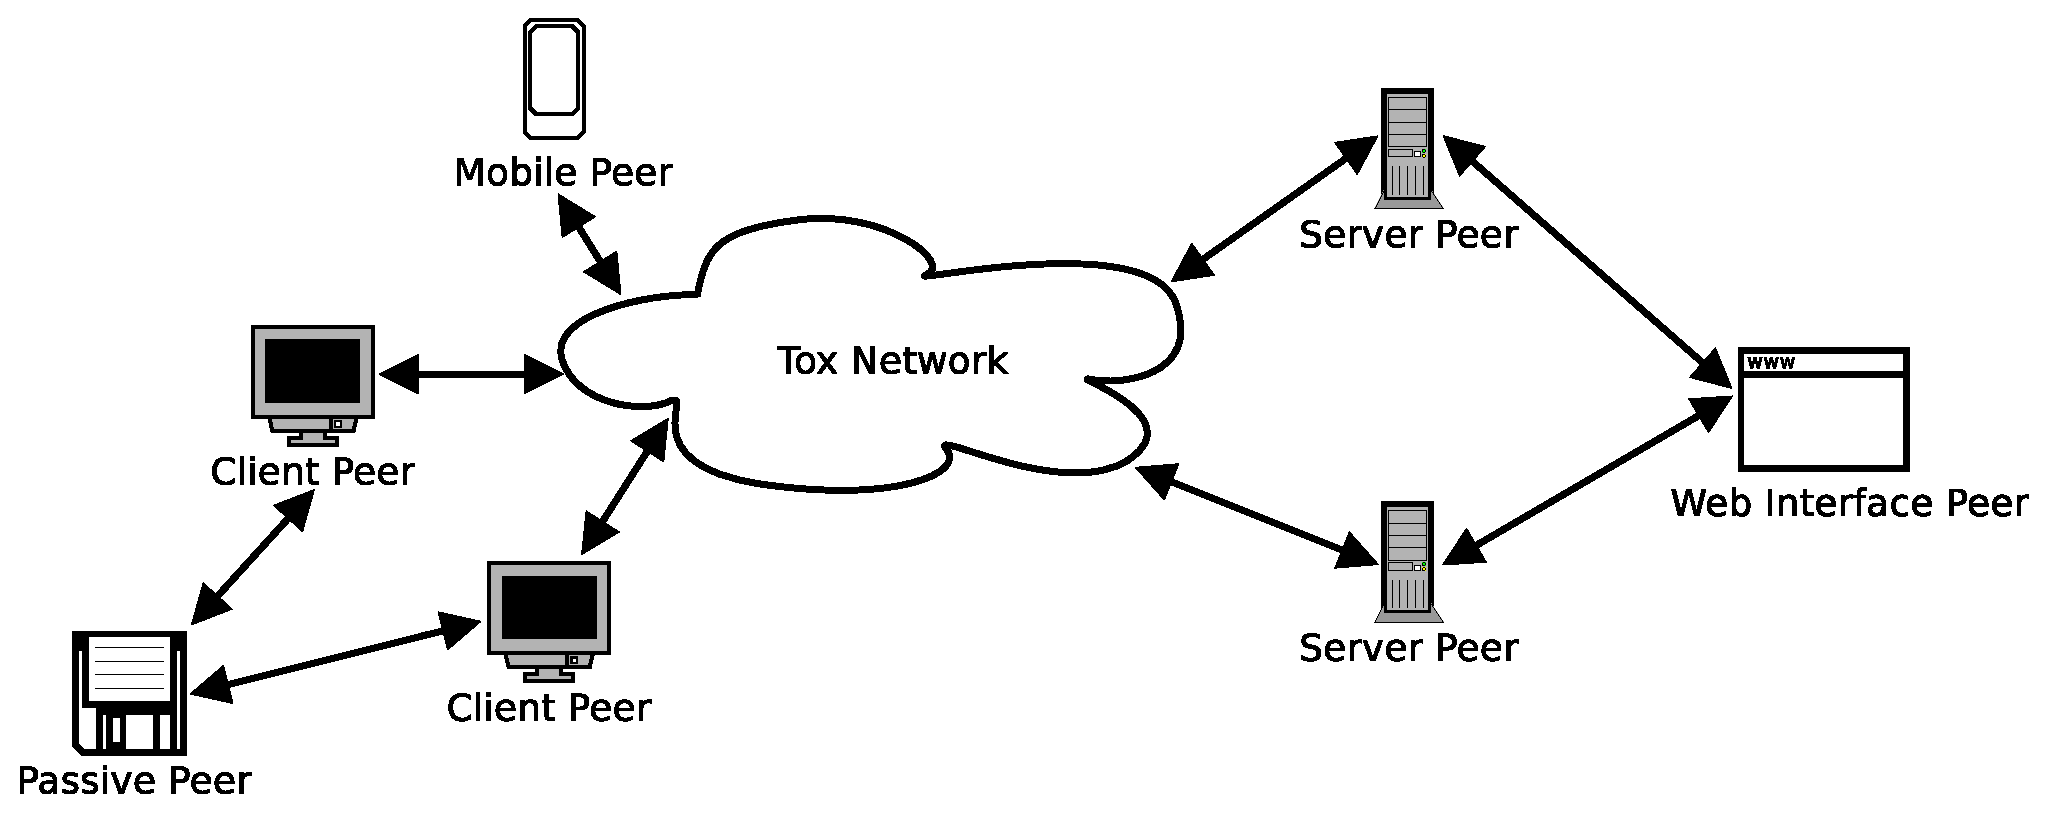
\includegraphics[width=12cm]{diagram/topo_software}
\caption[Tinzenite Software Diagram]{Example Tinzenite network with all proposed possible clients. Note that not all clients communicate via the underlying Tox communication network.}
\label{fig:software}
\end{figure}

This section is dedicated to differentiating the possible client applications we will implement as reference implementations.
Figure~\ref{fig:software} shows an overview of how the various parts could mesh together to form a complete Tinzenite network.
Note that the exact feature set is to be determined by the required development time of each feature and thus might lead to some features or even complete clients not being implemented for the thesis.
Those features can be implemented at a later time if so desired and will thus be referenced in the future work (see section~\ref{sec:Future Work}).

\subsection{Tinzenite Core Library}
\label{sub:Tinzenite Core Library}

The Tinzenite core library is the central reference implementation of the protocol.
It builds directly on the Tox core library and wraps the complete communication of Tinzenite.
Programs that implement the provided functionality will attach callbacks and call public methods to interface with it.
The library will also handle watching a specified directory on disk.
If the user modifies the contents of the directory that is watched by the library it will update its internal model and start trying to synchronize the changes to other peers.

To keep development of clients as easy as possible while at the same time keeping the protocol consistent between them we will separate the core logic for Tinzenite from any user oriented code.
This will ensure a maximum of adaptability for clients, meaning that they will not be constrained by the cross platform capabilities of the library itself.
The only limiting factor for porting the library to other platforms is the availability of the required Tox core library beneath it.

\subsection{Client Peer}

The basic client peer will be developed first and serve to validate the protocol.
This software will be the target of the user's primary interaction with the Tinzenite system.
Therefore we plan on including full coverage for required assistance in connecting peers and setting them up.
The client peer will always be a trusted peer and thus store the user's data in clear text on the disk.
Since the client peer will be the primary implemented peer, it will evolve directly with the core library.
Advanced features that may be implemented include but are not limited to support for shadow files and a low system footprint so that the client software can be run continuously without negatively impacting the operating system performance.
From the user's point of view the client software will provide an interface to connect to and accept new and existing peers.

\subsection{Server Peer}

The second dedicated software to be developed is the server peer.
This software will implement an encrypted peer for the Tinzenite network.
As the task of encrypting data falls to the trusted peer before uploading said data, the server peer must only offer a simple key value storage system for writing the encrypted data somewhere where it can later be retrieved.
Thus the encrypted peer allows clients to offer a storage interface and will use that instead of writing via a self specified method.

As a proof of concept that this is going to work we will develop two instances of such a storage interface.
The first one will be a simple store and retrieval to the local disk where the encrypted peer is running.
The other one will utilize the Hadoop file system to offer an example of a large scale distributed storage system as it might be used on an actual server for multiple users.

Unlike the client peer however we do not require user interfaces and file watchers.
Since the encrypted peer must only be started and connected to an existing network, no further user interaction than those two operations are required.
A file watcher like the client peer is not required because updates can not originate from the encrypted data set.
These encrypted peers will also utilize a different subset of the communication protocol as they operate essentially as blind data dumps.

\subsection{Web Interface Peer}
\label{sub:Web Interface Peer}

Built on top of an encrypted server peer it should theoretically be possible to implement access to the encrypted data for the user via a web interface.
This can be realized by allowing users to enter their password which in turn unlocks the decryption keys required to decrypt the stored data.
By utilizing client side code within a web browser, these operations can be done without involving the server peer beyond its use as a blind data store.
This peer would require a Javascript implementation of the Tinzenite protocol.
Golang can be compiled to Javascript~\cite{web:site:github:gopherjs} which should allow at least some reuse of existing code.

\subsection{Mobile Peer}

Nowadays no software is complete without a complimenting mobile application.
Thus Tinzenite should also offer a mobile client for the Android platform~\cite{web:site:android}.
Apart from the specific touchscreen oriented interface this peer would prove that Tinzenite can run on mobile platforms.
This would build on Golang's cross platform support even for Android~\cite{web:site:golang:mobile}.
Further work may be done here to ensure that Tinzenite runs in a mobile friendly way.
This implies low power consumption and low bandwidth capabilities.
Therefore support for shadow files and deltas is almost strictly required to meet the needs of a mobile peer.
When first using the mobile peer for the first time it may even be beneficial to ask the user whether the mobile peer should pull all data or just immediately mark everything as shadow objects, thus requiring the user to mark files manually to be fetched locally but reducing bandwidth requirements enormously.

\subsection{Passive Peer}

While not in itself a program, support for blind data dumps as passive peers is another aspect for which Tinzenite could be expanded to include support for.
This feature would require of Tinzenite to run the base encrypted peer logic on a given directory without the communication aspect via Tox.
These passive peers would allow easy backups of directories on passive storage media that can be easily updated by connecting it to an active peer.
